\begin{figure}
	\centering
	\begin{minipage}{.5\textwidth}
	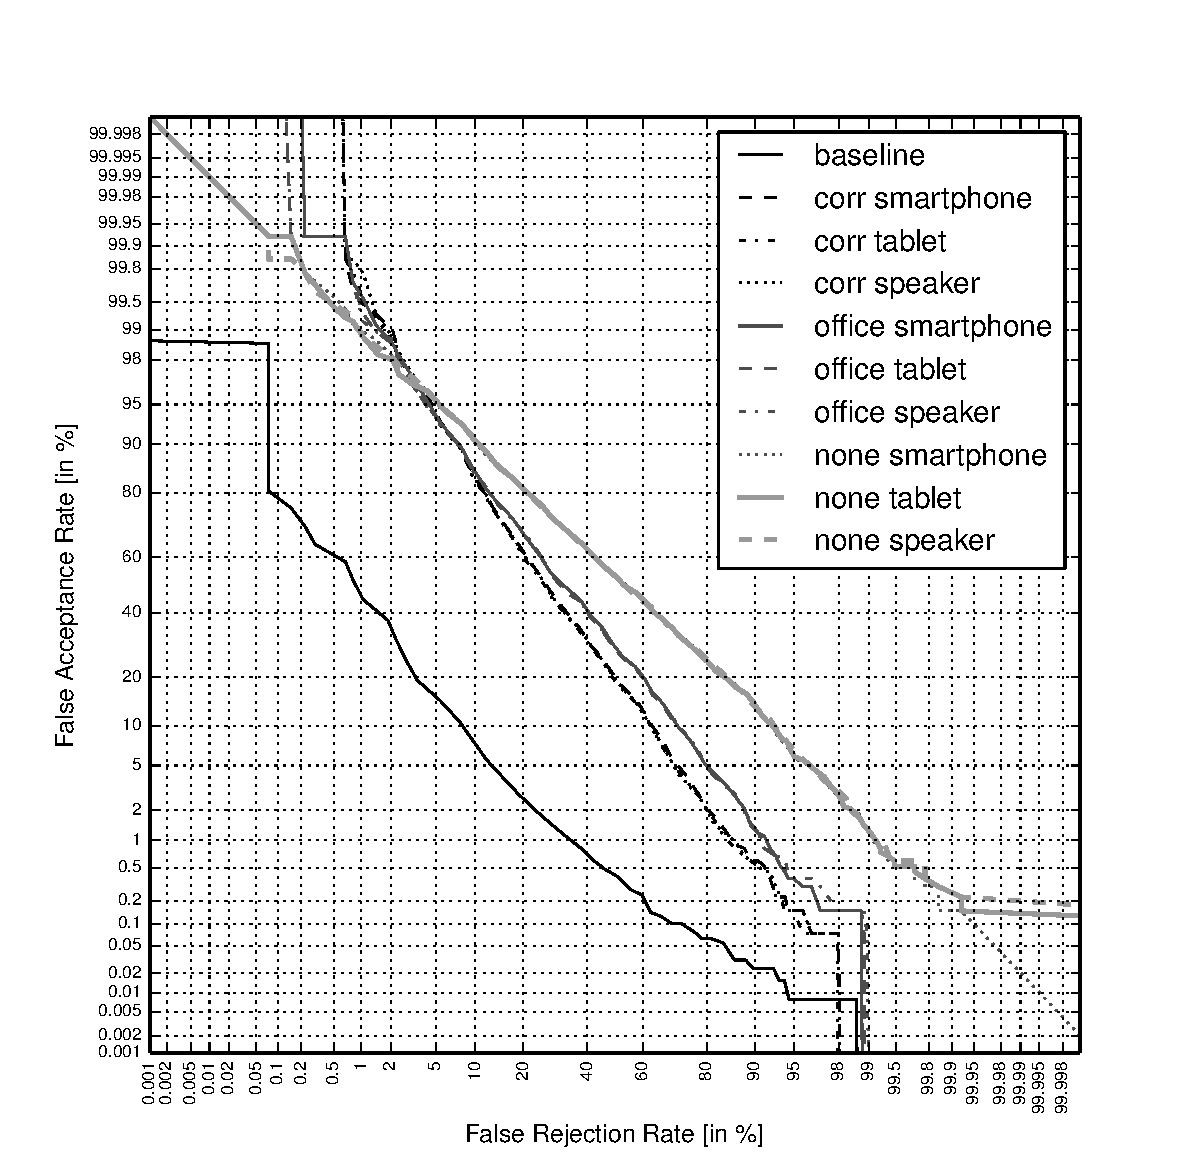
\includegraphics[width=1\linewidth]{Figs/DETs_GMM.pdf}
	\caption{DET plots for the GMM-UBM system for various replay configurations, compared to the baseline performance.}
	\label{fig::DETs_replay_GMM}
	\end{minipage}
	\begin{minipage}{.5\textwidth}
	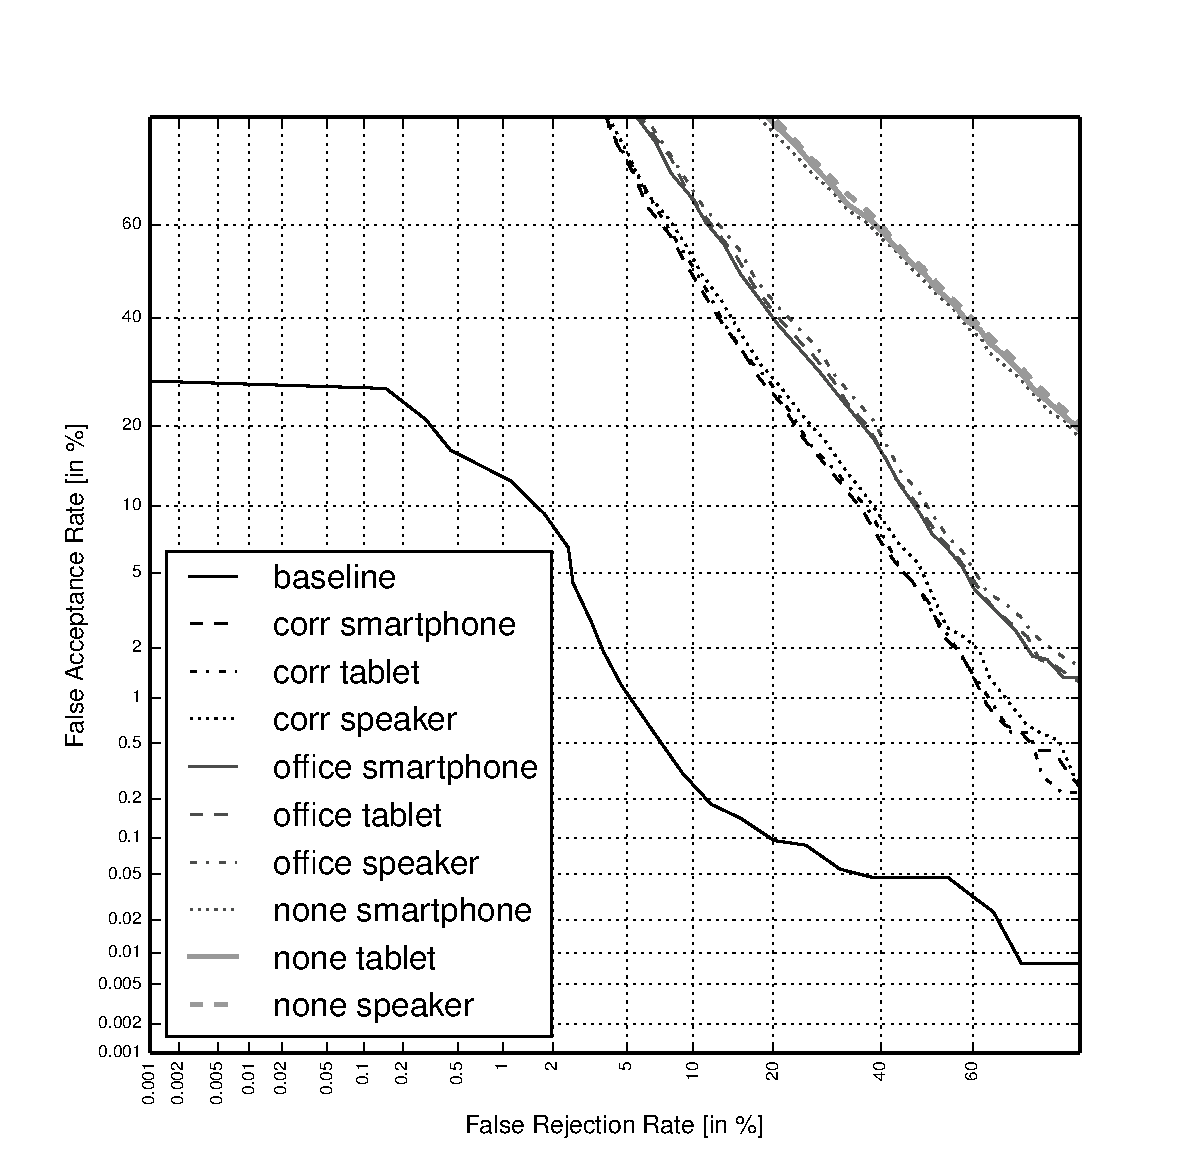
\includegraphics[width=1\linewidth]{Figs/DETs_IV.pdf}
	\caption{DET plots for the IV-PLDA system for various replay configurations, compared to the baseline performance.}
	\label{fig::DETs_replay_IV}
	\end{minipage}


\end{figure}



\begin{figure}
	\centering
	\begin{minipage}{.5\textwidth}
	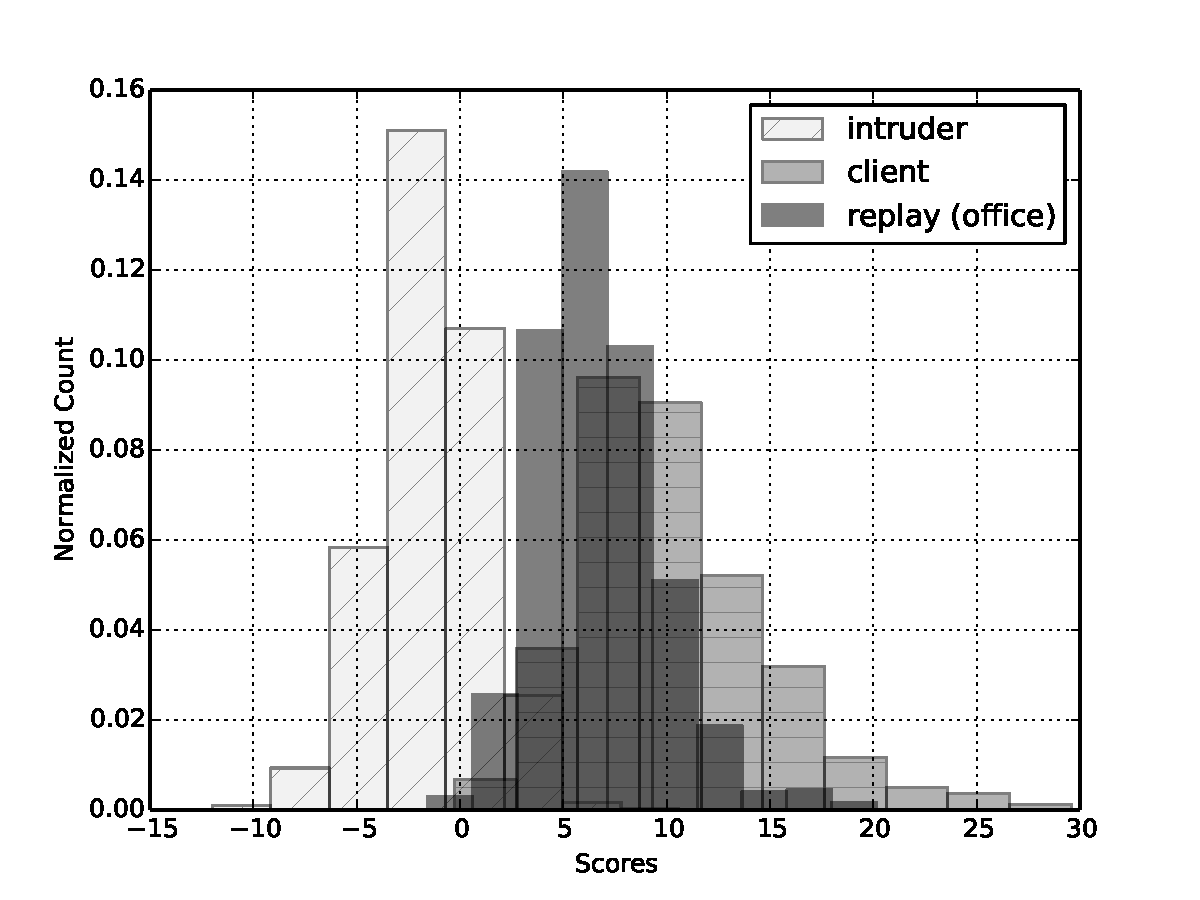
\includegraphics[width=1\linewidth]{Figs/dist_IV_off.pdf}
	\end{minipage}

%	\begin{minipage}{0.5\textwidth}
%	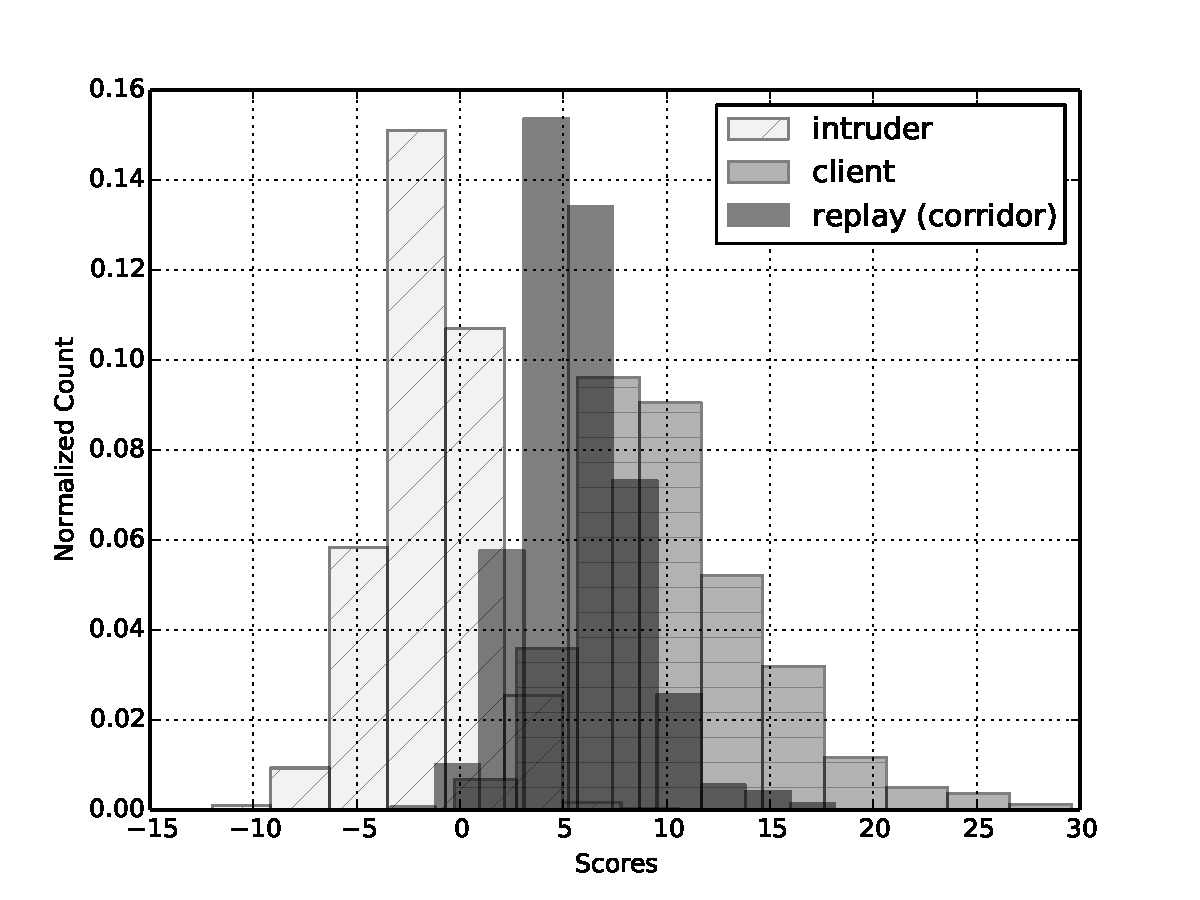
\includegraphics[width=1\linewidth]{Figs/dist_IV_corr.pdf}
%	\end{minipage}
%
%	\begin{minipage}{0.5\textwidth}
%	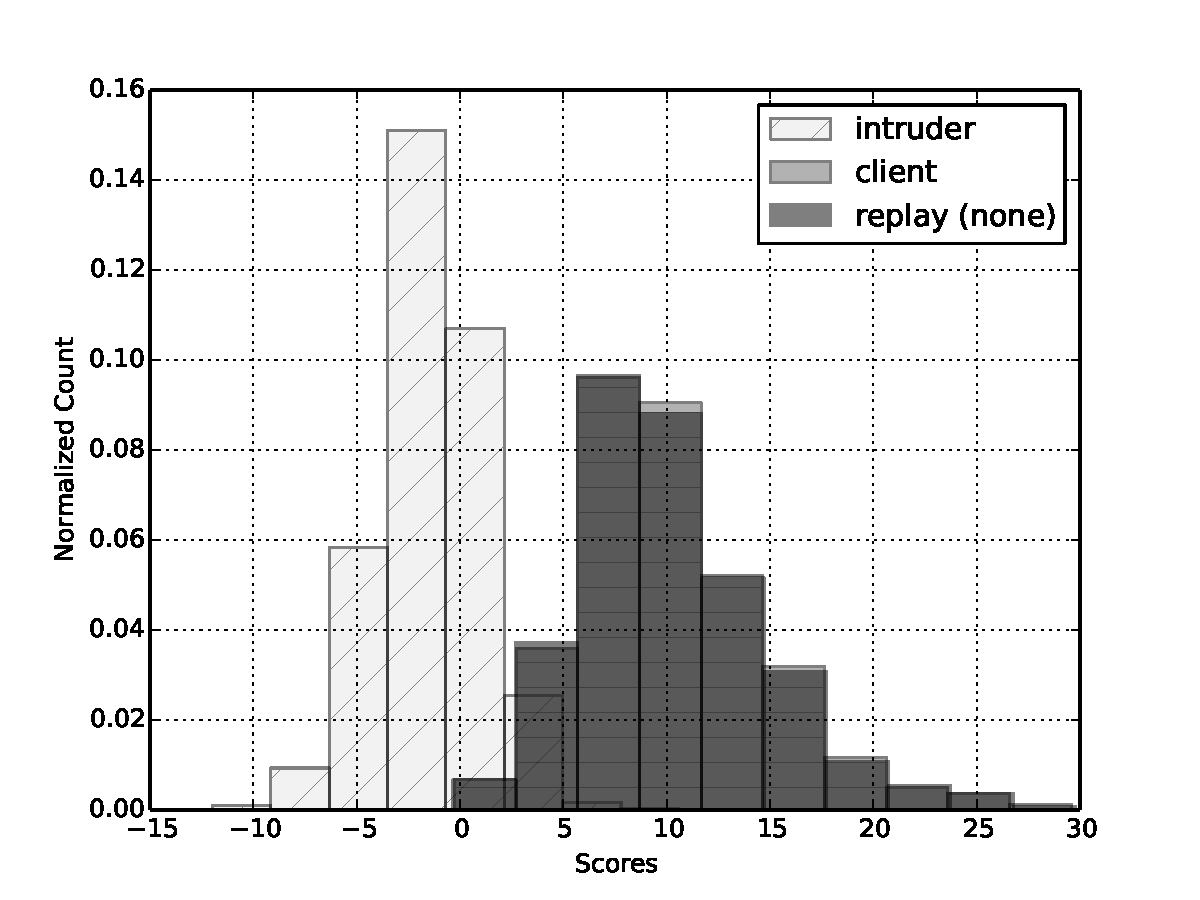
\includegraphics[width=1\linewidth]{Figs/dist_IV_none.pdf}
%	\end{minipage}

	\caption{Score distribution for the IV-PLDA system for replay attacks using a stand-alone speaker and emulation of an office.}
	\label{fig::Dist_IV}
\end{figure}

\subsubsection{FFD setup} The FFD countermeasure was set up according to the algorithm proposed in~\cite{Villalba2011}. 

The total modulation index was calculated based on the speech signal's envelope. The envelope was approximated by the absolute value of the signal downsampled to 60 Hz. The average modulation index of the signal was calculated for
the frames whose index was above a threshold of 0.75. 




\subsubsection{LBP setup} 


Compared to the original implementation, we reduced the number of possible patterns according to the standard Uniform LBP approach. Uniform LBPs are the subset of $58$ patterns which contain at most two bitwise transitions from 0 to 1 or 1 to 0 when the bit pattern is traversed in circularly fashion.  As an example, the subset includes patterns $00000001$ and $00111100$ but not $00110001$.  As reported by~\cite{Ojala2002}, most patterns are naturally uniform and empirical evidence suggests that their use in many image recognition applications leads to better performance then the full set of uniform and non-uniform patterns.  We observed similar findings in our previous work~\cite{Alegre2013a} and thus decided to ignore pixels corresponding to any of the 198 non-uniform patterns.

We used the implementation made publicly available by The University of Oulu\footnote{http://www.cse.oulu.fi/CMV/Downloads/LBPMatlab}. Normalised features used in the LBP countermeasure were composed of 51 coefficients: 16 LFCCs and energy plus their corresponding delta and delta-delta coefficients. We took into account only those frames determined to contain speech, i.e. those also used for ASV. Histograms of LBPs are created for all but the first and last frames, thereby obtaining a $58 \times 49 = 2842$ length feature vector.

\subsubsection{Training the replay detectors} Both countermeasure algorithms were trained using a set of 1000 recordings generated using 200 recordings taken from NIST'05 and emulation of various acoustic conditions. In order to make the experiment as close as possible to reality, we decided to use different room impulse responses than the ones used for simulation of replay attack. Therefore we emulated the following environment:
\begin{itemize}
\item a lecture room, with concrete walls, glass windows and a parquet;
\item a staircase, with concrete walls and steps;
\item a meeting room, with concrete walls, glass windows and a carpet.
\end{itemize}

Similarly to emulation of replay attack, the corresponding impulse responses were taken from the AIR database. To train the far-field recording detector, we also needed to emulate the replay device. We chose a stand-alone speaker impulse response, different from the one used for replay attack emulation, to avoid overfitting to testing data. Original NIST'05 recordings were used to model the licit client access trials.

A binary SVM classifier with polynomial kernel of 3rd degree was used for data classification for the FFD countermeasure, while a classifier based on decision table was used for LBP. Those classifiers returned the best results for those two detectors in terms of the area under the ROC curve. Having been trained, both classifiers were applied to detect replay attacks in both spoofing accesses and licit client trials.
